\section*{Learning rate optimisation}

2018/07/23 - SYNALP - Esteban MARQUER

\subsection{General information}

Learning rate is an hyperparameter in the training algorithm which
changes the speed of the training and the performance of the model.
Specifically, it is a coefficient of the gradient used to update the
parameters of the model.

There are three main learning rates for a model:
\begin{itemize}
\item a learning rate that is too small (closer to 0): the training is slow, and can get blocked in some local minima;
\item a learning rate that is too high (closer to +infinity, usually closer to 1): the learning is faster and avoid local minima, but could diverge from the solution;
\item a balanced learning rate: what we want to find, the traing is fast yet does not diverge.
\end{itemize}

\subsection{Optimisation process}

Usually, learning rate optimisation is done with a logarithmic scale of
the learning rate. The shape of the produced curves confirm the use of
such a scale.

The optimisation process is driven by three parameters and a single
metric.

The metric is the accuracy of the model on the validation corpus at the
end of the training.

The parameters are: the two bounds of the learning rate, and the
learning rate variation factor: the ``learning rate multiplier''.

The learning rate varies as follow in the psedo-python algorythm:

\begin{lstlisting}[language=Python]
# the learning rate takes the highest value as start value, as it will decrease over time
learning_rate = start_value 

# until the learning rate as reach the stop value (the lowest of the two bounds), we make it vary logarithmically
while learning_rate > stop_value:
    performance = train_model(learning_rate)
    save_model_performance(performance, learning_rate)
    
    # the learning rate is updated
    # example with a learning rate of 1 and a learning rate multiplier of 0.1:
    # at first the learning rate is 1, then 0.1, then 0.01 ...
    learning_rate = learning_rate * learning_rate_multiplier

# we compare the performance of the model with the different learning rates
compare_model_performance()
\end{lstlisting}

The closer to 0 the learning rate multiplier is, the faster the
variation will be, and the closer to 1 it si, the slower the variation
will be. To have a decent resolution in the curves, a multiplier close
to 1 is crucial.

The training is done each time on a full epoch.

\subsection{Results}

The first plot is done with a learning rate between 1 and 10\^{}(-5),
with a multiplier of 0.2. The second one is done with a learning rate
between 1 and 10\^{}(-2), with a multiplier of 0.6 (the total of dots is
10).

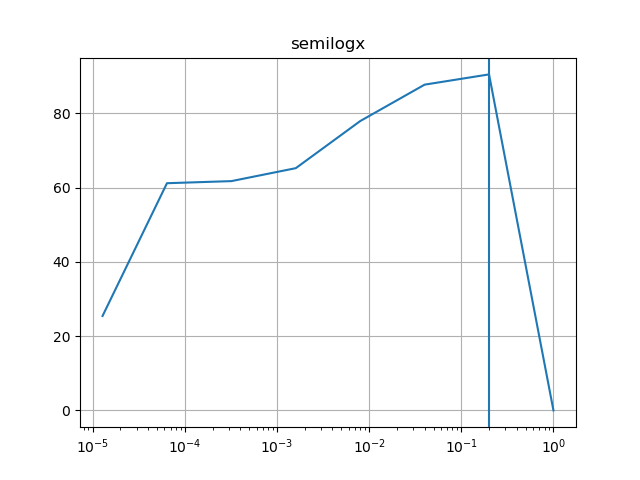
\includegraphics{parts/appendix/reports-papud/2018_07_23-Learning_rate_optimisation/lr_epoch_1_mul_0_2.png}
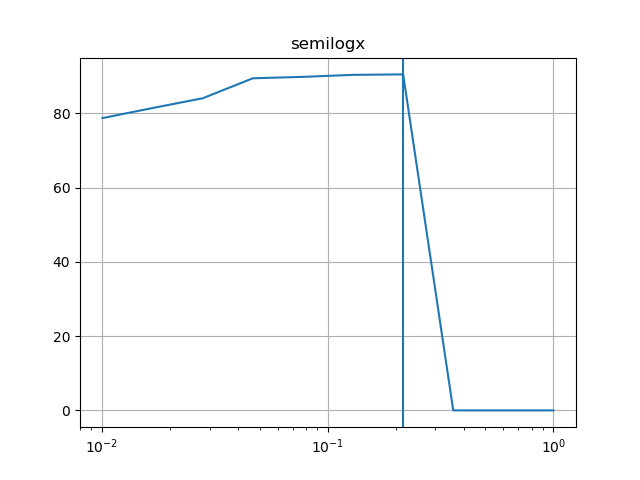
\includegraphics{parts/appendix/reports-papud/2018_07_23-Learning_rate_optimisation/lr_epoch_1_mul_0_6_best_0_216.png}

There is a strange accuracy at the end of the first plot: the
theoretically unreachable 0\%. It is confirmed by the second plot, with
multiple points having an accuracy of 0\%. With a baseline accuracy of
44\%, it is clear that the result diverge from wat is expected. It is a
case of divergence due to a learning rate that is too high.

The best learning rate found is 0.216 (0.6\^{}3), giving the fastest
learning (over 90\% of accuracy in 1 epoch) without diverging.

\subsection{Additional information}

The current implementation consist of a script building a model, and
finding the ideal learning rate for this model. It is an offline
implementation of the model.

The way it is implemented is ideal for an online use too, as the only
operation needed are the removal of the plotting part, and adding the
reload of the model with an updated learning rate.

\subsection{Improvements and next
steps}

Use the new learning rate in the training. As it is quite close to
diverge, it would be advised to use a slightly lower learning rate like
0.2.

If inline optimisation is used, three possibilities seem viable: -
choosing the learning rate every time we start a training, to adapt to
the current hyperparameters; - updating the learning rate every set
number of epochs, to adapt the learning to the current state of the
model; - doing each epoch with a set of learning rates, and every time
choosing the best result; even if costly (every epoch is done multiple
time), it should allow a really fast learning with lowered chances of
divergence or over-fitting.

Personally, my preferred option is the second one.
